%%%%%%%%%%%%%%%%%%%%%%%%%%%%%%%%%%%%%%%%%
% Lachaise Assignment
% LaTeX Template
% Version 1.0 (26/6/2018)
%
% This template originates from:
% http://www.LaTeXTemplates.com
%
% Authors:
% Marion Lachaise & François Févotte
% Vel (vel@LaTeXTemplates.com)
%
% License:
% CC BY-NC-SA 3.0 (http://creativecommons.org/licenses/by-nc-sa/3.0/)
% 
%%%%%%%%%%%%%%%%%%%%%%%%%%%%%%%%%%%%%%%%%

%----------------------------------------------------------------------------------------
%	PACKAGES AND OTHER DOCUMENT CONFIGURATIONS
%----------------------------------------------------------------------------------------

\documentclass{article}
\usepackage{enumitem}
\usepackage{dsfont}
\usepackage{graphicx}
%%%%%%%%%%%%%%%%%%%%%%%%%%%%%%%%%%%%%%%%%
% Lachaise Assignment
% Structure Specification File
% Version 1.0 (26/6/2018)
%
% This template originates from:
% http://www.LaTeXTemplates.com
%
% Authors:
% Marion Lachaise & François Févotte
% Vel (vel@LaTeXTemplates.com)
%
% License:
% CC BY-NC-SA 3.0 (http://creativecommons.org/licenses/by-nc-sa/3.0/)
% 
%%%%%%%%%%%%%%%%%%%%%%%%%%%%%%%%%%%%%%%%%

%----------------------------------------------------------------------------------------
%	PACKAGES AND OTHER DOCUMENT CONFIGURATIONS
%----------------------------------------------------------------------------------------

\usepackage{amsmath,amsfonts,stmaryrd,amssymb} % Math packages

\usepackage{enumerate} % Custom item numbers for enumerations

\usepackage[ruled]{algorithm2e} % Algorithms

\usepackage[framemethod=tikz]{mdframed} % Allows defining custom boxed/framed environments

\usepackage{listings} % File listings, with syntax highlighting
\lstset{
	basicstyle=\ttfamily, % Typeset listings in monospace font
}

%----------------------------------------------------------------------------------------
%	DOCUMENT MARGINS
%----------------------------------------------------------------------------------------

\usepackage{geometry} % Required for adjusting page dimensions and margins

\geometry{
	paper=a4paper, % Paper size, change to letterpaper for US letter size
	top=2.5cm, % Top margin
	bottom=3cm, % Bottom margin
	left=2.5cm, % Left margin
	right=2.5cm, % Right margin
	headheight=14pt, % Header height
	footskip=1.5cm, % Space from the bottom margin to the baseline of the footer
	headsep=1.2cm, % Space from the top margin to the baseline of the header
	%showframe, % Uncomment to show how the type block is set on the page
}

%----------------------------------------------------------------------------------------
%	FONTS
%----------------------------------------------------------------------------------------

\usepackage[utf8]{inputenc} % Required for inputting international characters
\usepackage[T1]{fontenc} % Output font encoding for international characters

\usepackage{XCharter} % Use the XCharter fonts

%----------------------------------------------------------------------------------------
%	COMMAND LINE ENVIRONMENT
%----------------------------------------------------------------------------------------

% Usage:
% \begin{commandline}
%	\begin{verbatim}
%		$ ls
%		
%		Applications	Desktop	...
%	\end{verbatim}
% \end{commandline}

\mdfdefinestyle{commandline}{
	leftmargin=10pt,
	rightmargin=10pt,
	innerleftmargin=15pt,
	middlelinecolor=black!50!white,
	middlelinewidth=2pt,
	frametitlerule=false,
	backgroundcolor=black!5!white,
	frametitle={Command Line},
	frametitlefont={\normalfont\sffamily\color{white}\hspace{-1em}},
	frametitlebackgroundcolor=black!50!white,
	nobreak,
}

% Define a custom environment for command-line snapshots
\newenvironment{commandline}{
	\medskip
	\begin{mdframed}[style=commandline]
}{
	\end{mdframed}
	\medskip
}

%----------------------------------------------------------------------------------------
%	FILE CONTENTS ENVIRONMENT
%----------------------------------------------------------------------------------------

% Usage:
% \begin{file}[optional filename, defaults to "File"]
%	File contents, for example, with a listings environment
% \end{file}

\mdfdefinestyle{file}{
	innertopmargin=1.6\baselineskip,
	innerbottommargin=0.8\baselineskip,
	topline=false, bottomline=false,
	leftline=false, rightline=false,
	leftmargin=2cm,
	rightmargin=2cm,
	singleextra={%
		\draw[fill=black!10!white](P)++(0,-1.2em)rectangle(P-|O);
		\node[anchor=north west]
		at(P-|O){\ttfamily\mdfilename};
		%
		\def\l{3em}
		\draw(O-|P)++(-\l,0)--++(\l,\l)--(P)--(P-|O)--(O)--cycle;
		\draw(O-|P)++(-\l,0)--++(0,\l)--++(\l,0);
	},
	nobreak,
}

% Define a custom environment for file contents
\newenvironment{file}[1][File]{ % Set the default filename to "File"
	\medskip
	\newcommand{\mdfilename}{#1}
	\begin{mdframed}[style=file]
}{
	\end{mdframed}
	\medskip
}

%----------------------------------------------------------------------------------------
%	NUMBERED QUESTIONS ENVIRONMENT
%----------------------------------------------------------------------------------------

% Usage:
% \begin{question}[optional title]
%	Question contents
% \end{question}

\mdfdefinestyle{question}{
	innertopmargin=1.2\baselineskip,
	innerbottommargin=0.8\baselineskip,
	roundcorner=5pt,
	nobreak,
	singleextra={%
		\draw(P-|O)node[xshift=1em,anchor=west,fill=white,draw,rounded corners=5pt]{%
		Question \theQuestion\questionTitle};
	},
}

\newcounter{Question} % Stores the current question number that gets iterated with each new question

% Define a custom environment for numbered questions
\newenvironment{question}[1][\unskip]{
	\bigskip
	\stepcounter{Question}
	\newcommand{\questionTitle}{~#1}
	\begin{mdframed}[style=question]
}{
	\end{mdframed}
	\medskip
}

%----------------------------------------------------------------------------------------
%	WARNING TEXT ENVIRONMENT
%----------------------------------------------------------------------------------------

% Usage:
% \begin{warn}[optional title, defaults to "Warning:"]
%	Contents
% \end{warn}

\mdfdefinestyle{warning}{
	topline=false, bottomline=false,
	leftline=false, rightline=false,
	nobreak,
	singleextra={%
		\draw(P-|O)++(-0.5em,0)node(tmp1){};
		\draw(P-|O)++(0.5em,0)node(tmp2){};
		\fill[black,rotate around={45:(P-|O)}](tmp1)rectangle(tmp2);
		\node at(P-|O){\color{white}\scriptsize\bf !};
		\draw[very thick](P-|O)++(0,-1em)--(O);%--(O-|P);
	}
}

% Define a custom environment for warning text
\newenvironment{warn}[1][Warning:]{ % Set the default warning to "Warning:"
	\medskip
	\begin{mdframed}[style=warning]
		\noindent{\textbf{#1}}
}{
	\end{mdframed}
}

%----------------------------------------------------------------------------------------
%	INFORMATION ENVIRONMENT
%----------------------------------------------------------------------------------------

% Usage:
% \begin{info}[optional title, defaults to "Info:"]
% 	contents
% 	\end{info}

\mdfdefinestyle{info}{%
	topline=false, bottomline=false,
	leftline=false, rightline=false,
	nobreak,
	singleextra={%
		\fill[black](P-|O)circle[radius=0.4em];
		\node at(P-|O){\color{white}\scriptsize\bf i};
		\draw[very thick](P-|O)++(0,-0.8em)--(O);%--(O-|P);
	}
}

% Define a custom environment for information
\newenvironment{info}[1][Info:]{ % Set the default title to "Info:"
	\medskip
	\begin{mdframed}[style=info]
		\noindent{\textbf{#1}}
}{
	\end{mdframed}
}
 % Include the file specifying the document structure and custom commands

%----------------------------------------------------------------------------------------
%	ASSIGNMENT INFORMATION
%----------------------------------------------------------------------------------------

\title{QF602 Derivatives: Homework \#3} % Title of the assignment

\author{ChanJung Kim} 

\date{\today} % University, school and/or department name(s) and a date

%----------------------------------------------------------------------------------------

\begin{document}
	
	\maketitle % Print the title
	
	\section*{Part 3 - Convexity Correction} % Numbered section
	
	\subsection*{Present value of CMS product}	
	\noindent To calculate PV of leg receiving CMS10y semi-annually over the next 5 years, we need to find SABR paramters at different expiries in order to price each CMS rate. To this end, cubic spline interpolation is used between $\alpha$ $\nu$, and $\rho$ of $1y$ $\times$ $10y$, $5y\times10y$ and $10y\times10y$ SABR models we have calibrated. Since there was no expiry lower than 1y for us to interpolate, parameters for 0.5y expiry follows those of 1y expiry.\\
	
	\noindent Interpolation profiles are given as follow:\\
	
	\begin{figure}[h]
	\centering
	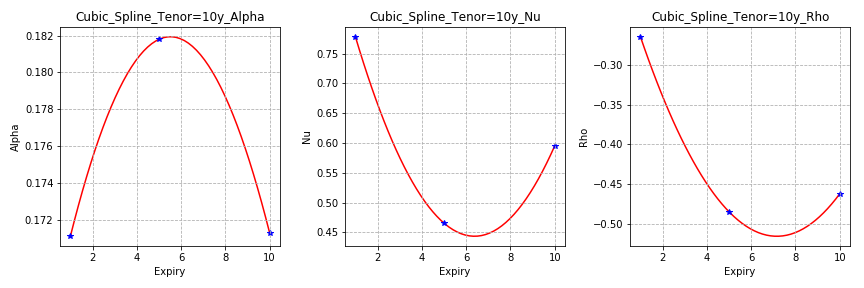
\includegraphics[scale=0.5]{Cubic_10y.png}
	\caption{Interpolation of SABR parameters - CMS10Y}
	\end{figure}	
	
	\noindent After interpolating all the SABR parameters, static replication is used to price each CMS rate and PV is the sum of the discounted values of all CMS rates, multiplied by the day count fraction. Here goes the mathematical form:
	\begin{align*}
	PV_{CMS10y}&=D(0,6m)\times 0.5 \times E^T [S_{6m,10y6m}(6m)] \\&+ D(0,1y) \times 0.5 \times E^T [S_{1y,11y}(1y)]\\&+ \dots 
	+D(0,5y) \times 0.5 \times E^T [S_{5y,15y}(5y)]\\&= 0.213606
	\end{align*}
	
	
	
	\noindent Similarly, for CMS2y processed quarterly, $\alpha$ $\nu$, and $\rho$ can be interpolated between $1y$ $\times$ $2y$, $5y\times2y$,$10y\times2y$, whose profiles are demonstrated below:\\ 
	
	\begin{figure}[h]
	\centering
	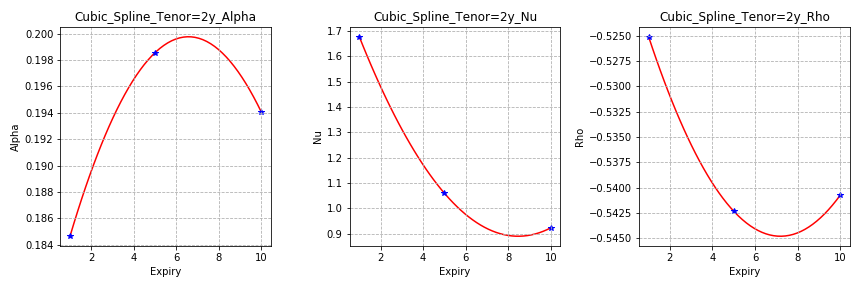
\includegraphics[scale=0.5]{Cubic_2y.png}
	\caption{Interpolation of SABR parameters - CMS2Y}
	\end{figure}	
	
	\noindent In addition to SABR parameters interpolation, due to quarterly arrangement, more discrete OIS discount rates and Libor discount rates are interpolated based on DF calculated in Section 1. After getting all the inputs, we can calculate PV of CMS2y as follow:
	\begin{align*}
	PV_{CMS2y}&=D(0,3m)\times 0.25 \times E^T [S_{3m,2y3m}(3m)] \\&+ D(0,6m) \times 0.25 \times E^T [S_{6m,2y6m}(6m)]\\&+ \dots 
	+D(0,10y) \times 0.25 \times E^T [S_{10y,12y}(10y)]\\&= 0.504841
	\end{align*}

	
	\subsection*{CMS VS Par Swap Rate}
	Through trial and error, we found out that the CMS rates can become unlikely large numbers or even drop below par swap rate when upper bound for payer swaption integral is set as a large number or infinity. To figure out the optimal upper bound that not only covers most of the cases but generates plausible CMS rates, we calculated pure $f(K)$ in CMS rate formula by setting the payoff function as constant 1. When the upper bound is 0.85, no value exceeded 1, and CMS rates converged on reasonable readings.

	\begin{figure}[h]
		\centering
		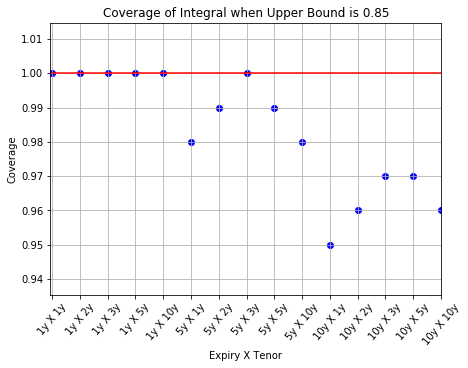
\includegraphics[scale=0.5]{Coverage.png}
		\caption{Coverage of Integral inside of CMS rate when Upper Bound is 0.85}
	\end{figure}
	
	Tables presented below show CMS rates for each maturity and tenor. 
	
	\begin{figure}[h]
		\centering
		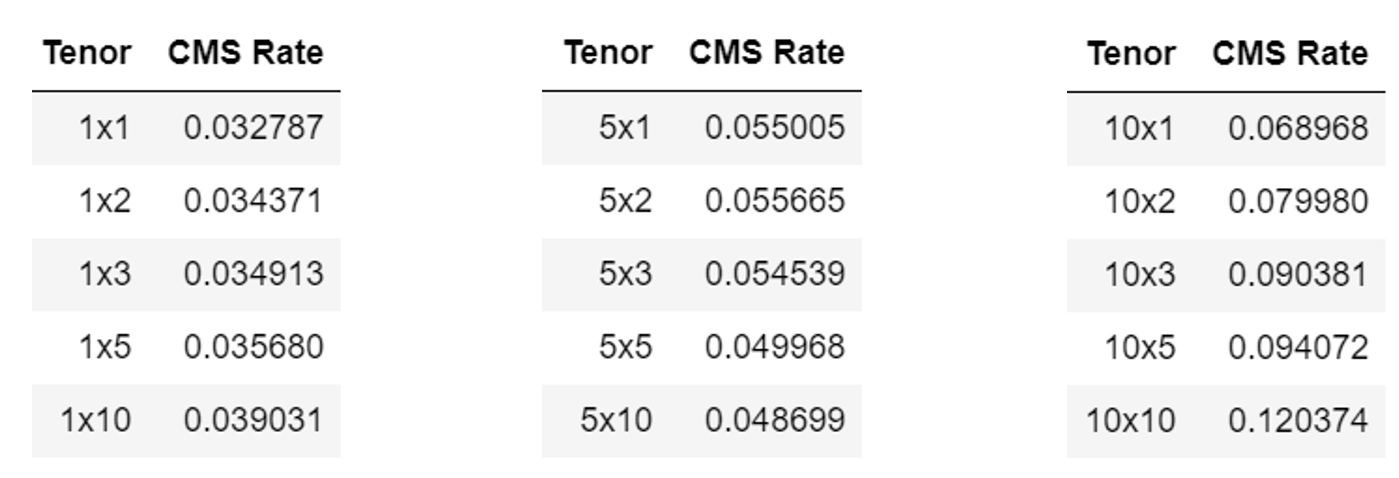
\includegraphics[scale=0.5]{CMS_RATE.png}
		\caption{CMS rates}
	\end{figure}
	
	\pagebreak
	
	 \noindent Comparing CMS rates with forward swap rates of corresponding expiry and tenor which are derived from Part 1, we can recognise that the difference between CMS and forward swap rate increases as the expiry lengthens. It means that the longer expiry becomes, the greater the magnitude of convexity correction grows. On the contrary, the influence of tenor on the convexity correction is irregular. This phenomenon is presumed to be a result of volatility smile. 

	\begin{figure}[ht]
		\centering
		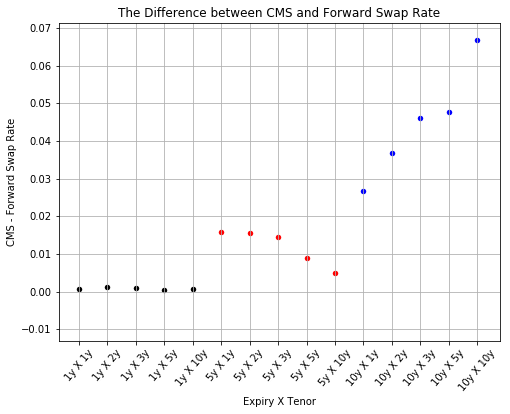
\includegraphics[scale=0.5]{CMS_FSR.png}
		\caption{Delta Profile for Up-and-In Barrier Option of Given Condition}
	\end{figure}



\end{document}